\begin{frame}{Lattice}
  \begin{tikzpicture}[remember picture,overlay]
    \fill [white] (current page.south west) rectangle (current page.north east);
    \node at (current page.center) {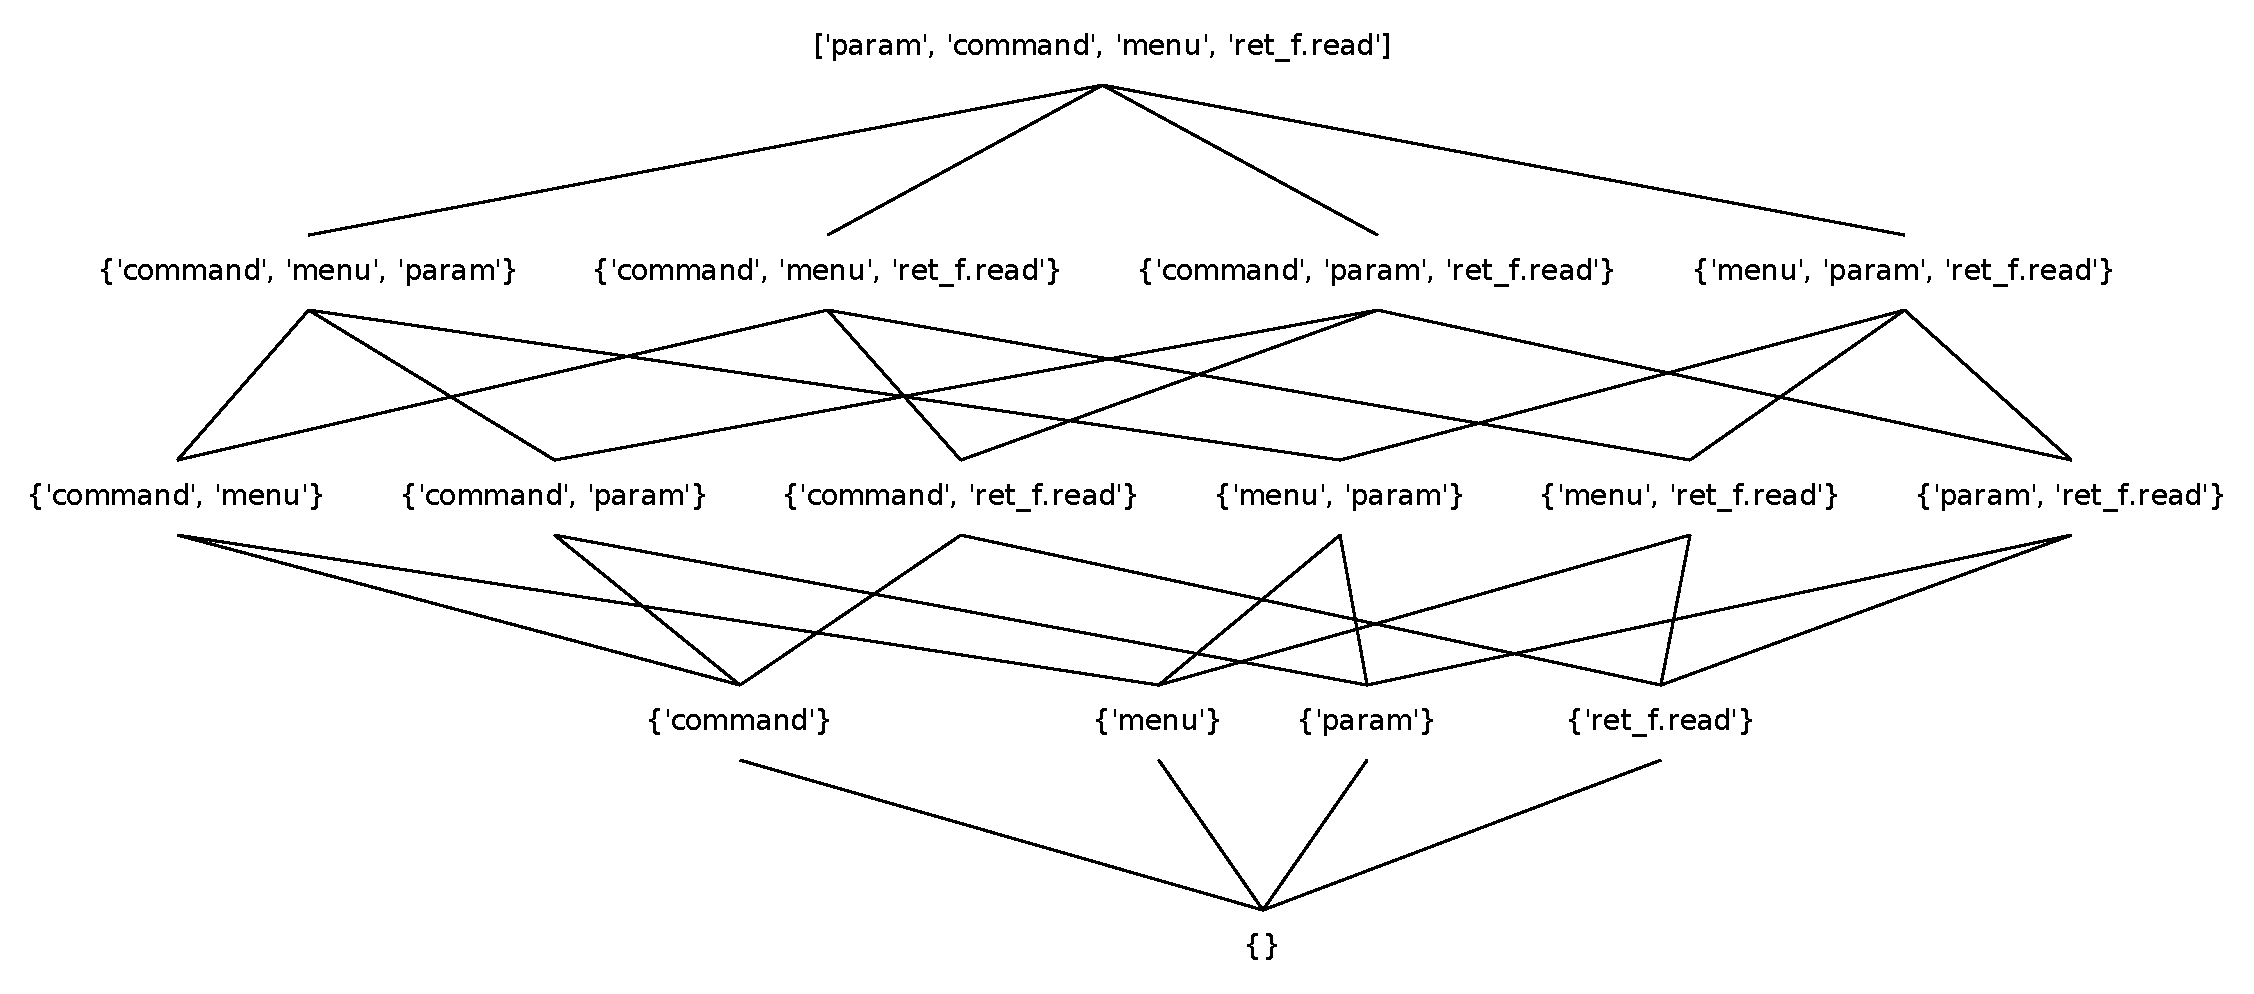
\includegraphics[width=1.1\textwidth]{graphics/command_injection_lattice}};
    \end{tikzpicture}
  
\end{frame}


\begin{frame}{Lattice}
  \begin{itemize}
  \item Partial order 
  \item Least upper bound for all subsets
  \item Greatest lower bound for all subsets
  \end{itemize}


  \begin{figure}
    \begin{subfigure}[b]{0.4\textwidth}
      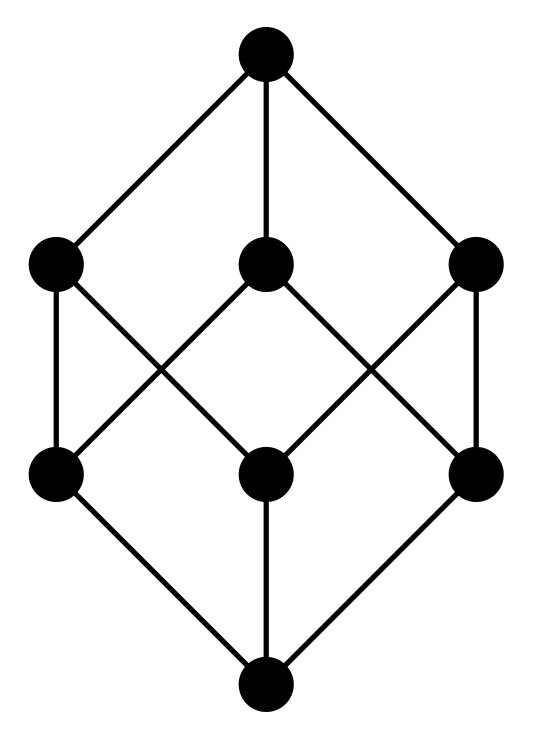
\includegraphics[width=0.6\textwidth]{graphics/lattice}
    \end{subfigure}
    ~
    \begin{subfigure}[b]{0.4\textwidth}
      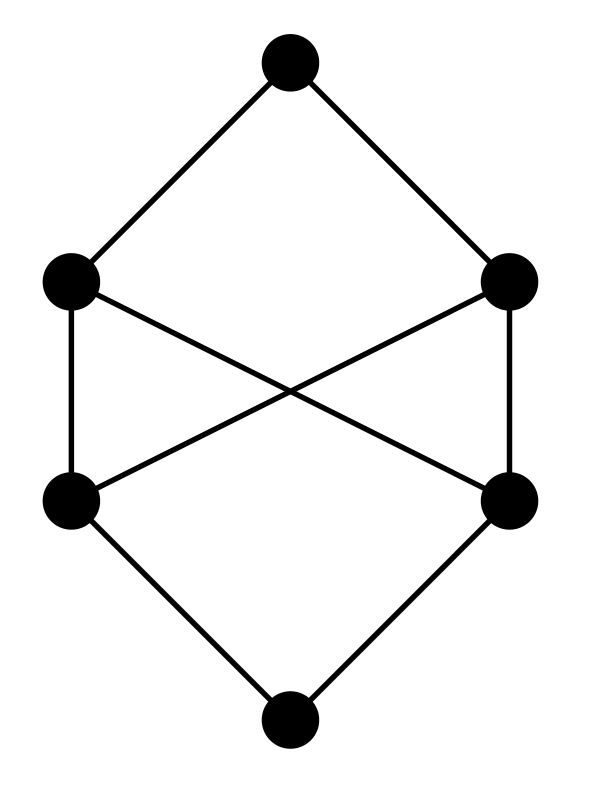
\includegraphics[width=0.6\textwidth]{graphics/notlattice}
    \end{subfigure}    
  \end{figure}
\end{frame}

\begin{frame}{Lattice}
  \begin{itemize}
  \item Partial order 
  \item Least upper bound for all subsets
  \item Greatest lower bound for all subsets
  \end{itemize}


  \begin{figure}
    \begin{subfigure}[b]{0.4\textwidth}
      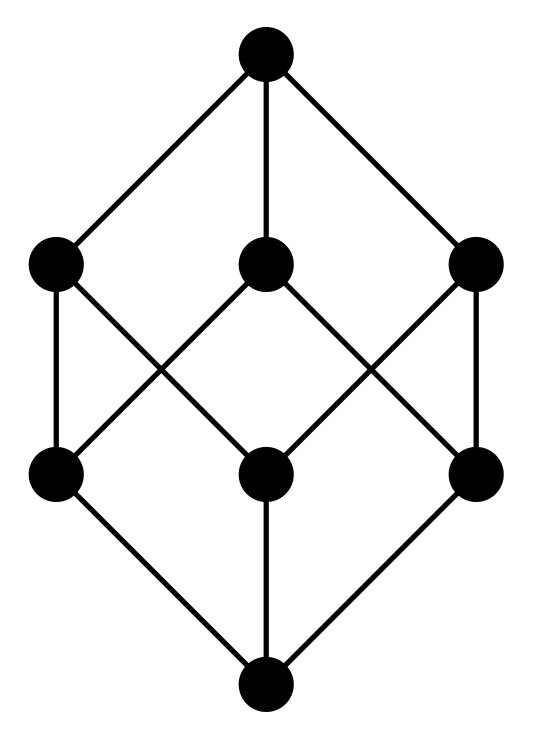
\includegraphics[width=0.6\textwidth]{graphics/lattice}
    \end{subfigure}
    ~
    \begin{subfigure}[b]{0.4\textwidth}
      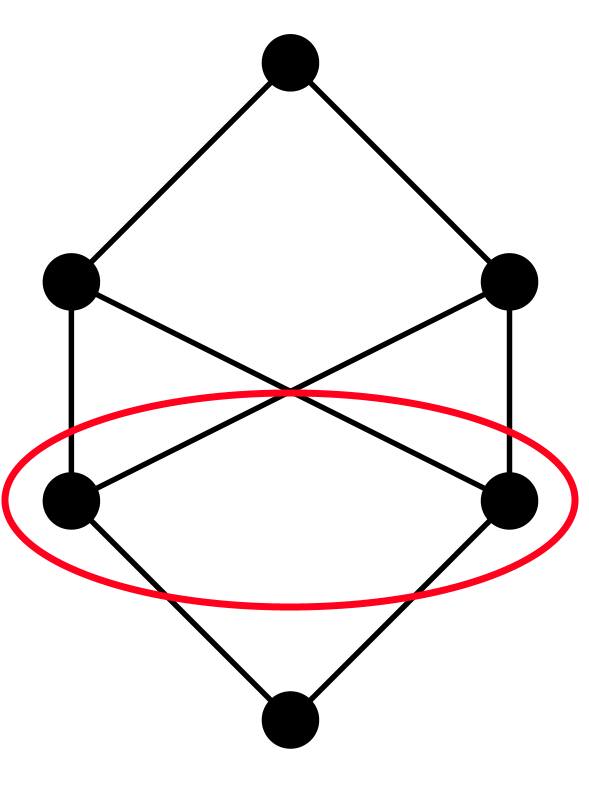
\includegraphics[width=0.6\textwidth]{graphics/notlatticepoints}
    \end{subfigure}    
  \end{figure}
\end{frame}

\begin{frame}{Lattice}
  \begin{itemize}
  \item Partial order 
  \item Least upper bound for all subsets
  \item Greatest lower bound for all subsets
  \end{itemize}


  \begin{figure}
    \begin{subfigure}[b]{0.4\textwidth}
      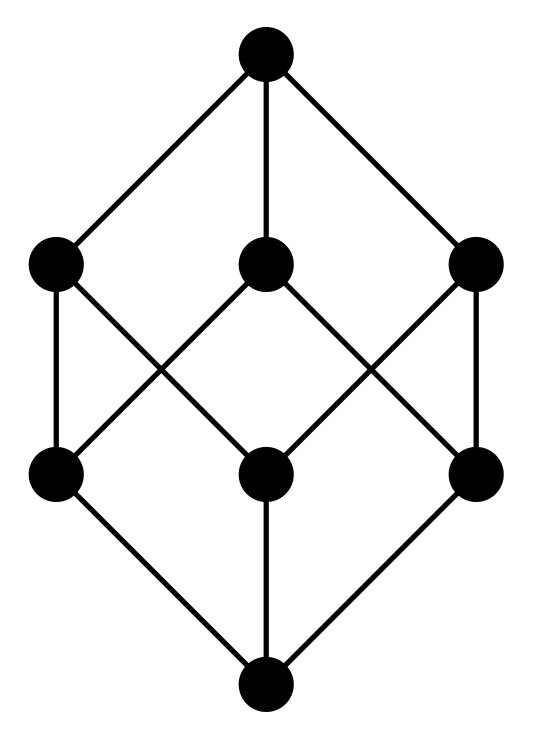
\includegraphics[width=0.6\textwidth]{graphics/lattice}
    \end{subfigure}
    ~
    \begin{subfigure}[b]{0.4\textwidth}
      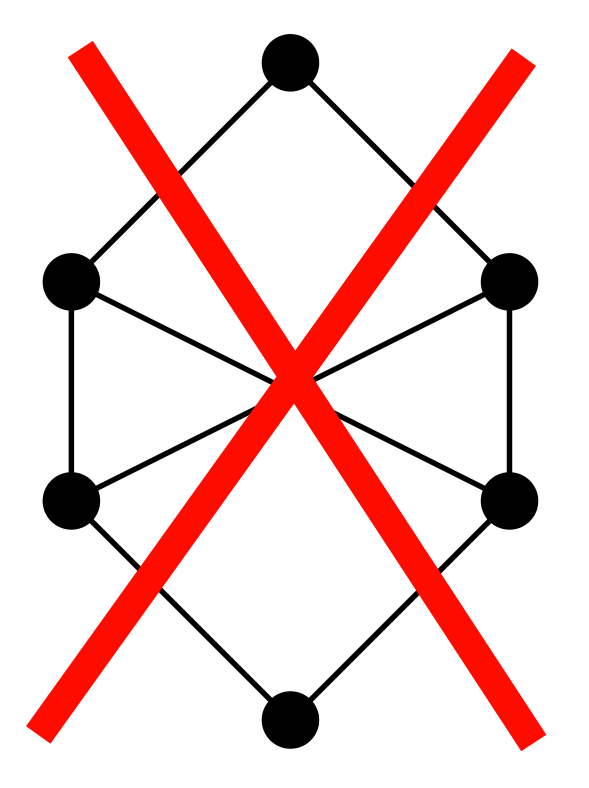
\includegraphics[width=0.6\textwidth]{graphics/definitelynotlattice}
    \end{subfigure}    
  \end{figure}
\end{frame}
